\documentclass[a4paper,12pt]{article} % тип документа

% Поля страниц
\usepackage[left=2.5cm,right=2.5cm, top=2cm,bottom=2cm,bindingoffset=0cm]{geometry}
    
%Пакет дял таблиц   
\usepackage{multirow} 
    
%Отступ после заголовка    
\usepackage{indentfirst}


% Рисунки
\usepackage{subcaption,floatrow,graphicx,calc}
\usepackage{wrapfig}

% Создаёем новый разделитель
\DeclareFloatSeparators{mysep}{\hspace{1cm}}

% Ссылки?
\usepackage{hyperref}
\usepackage[rgb]{xcolor}
\hypersetup{				% Гиперссылки
    colorlinks=true,       	% false: ссылки в рамках
	urlcolor=blue          % на URL
}


%  Русский язык
\usepackage[T2A]{fontenc}			% кодировка
\usepackage[utf8]{inputenc}			% кодировка исходного текста
\usepackage[english,russian]{babel}	% локализация и переносы


% Математика
\usepackage{amsmath,amsfonts,amssymb,amsthm,mathtools, mathrsfs, wasysym}


\begin{document}
\begin{center}
	\footnotesize{ФЕДЕРАЛЬНОЕ ГОСУДАРСТВЕННОЕ АВТОНОМНОЕ ОБРАЗОВАТЕЛЬНОЕ 			УЧРЕЖДЕНИЕ ВЫСШЕГО ОБРАЗОВАНИЯ}\\
	\footnotesize{МОСКОВСКИЙ ФИЗИКО-ТЕХНИЧЕСКИЙ ИНСТИТУТ\\(НАЦИОНАЛЬНЫЙ 			ИССЛЕДОВАТЕЛЬСКИЙ УНИВЕРСИТЕТ)}\\
	\footnotesize{ФАКУЛЬТЕТ ОБЩЕЙ И ПРИКЛАДНОЙ ФИЗИКИ\\}
	\hfill \break
	\hfill\break
	\hfill\break
	\hfill \break
	\hfill \break
	\hfill \break
	\hfill \break
	\hfill \break
	\hfill \break
	\hfill \break
	\hfill \break
	\hfill \break
	\hfill \break
	\hfill \break
	\large{Лабораторная работа № Д.4.4 \\\textbf{Определение длины волны лазера\\с помощью линейки}}\\
	\hfill \break
	\hfill \break
	\hfill \break
	\begin{flushright}
		Серебренников Даниил\\
		Группа Б02-826
	\end{flushright}
	\hfill \break
	\hfill \break
	\hfill \break
	\hfill \break
	\hfill \break
	\hfill \break
	\hfill \break
	\hfill \break
	\hfill \break
	\hfill \break
	\hfill \break
\end{center}
\begin{center}
	Долгопрудный, 2020 г.
\end{center}
\thispagestyle{empty}
\newpage
	\textbf{Цель работы:} знакомство с элементами юстировки оптической системы, работа с грубыми дифракционными решётками ($\lambda \ll d $), определение длины волны излучения лазера.

	\textbf{В работе используются:}  зелёный полупроводниковый лазер, металлическая линейка длиной 15 см, с полумиллиметровыми делениями, небольшое зеркальце, рулетка, скотч, ножницы, камера смартфона.
\section{Теоретическая часть}
	Дифракционные решётки, которые обычно используются для анализа спектров, имеют порядка $10^{3} - 10^{4}$ штрихов на сантиметр, т. е. имеют период, сравнимый с длиной волны $\lambda$ света видимого диапазона. 

	На грубых решётках ($\lambda \ll d $) из-за малых углов дифракции $\varphi \sim \frac{\lambda}{d}$ обнаружить  и, тем более, исследовать дифракционную картину крайне сложно. В этом случае эффективным оказывается использование скользящих лучей, когда угол падения близок к $\pi$.

	При наклонном падении лучей на дифракционную решётку условие дифракционного максимума $m$-го порядка имеет вид:
	\begin{equation*}
		d (\sin \varphi _{0} - \sin \varphi _{m}) = m\lambda.
	\end{equation*}
	В дальнейшем мы будем использовать не углы падения $\varphi$, а углы скольжения $\theta = \pi - \varphi$. Тогда, условие максимума перепишется в виде: 
	\begin{equation}
		\label{kek}
		\tag{*}
		d (\cos \theta _{0} - \cos \theta _{m}) = m\lambda.
	\end{equation}
	Для дифракционного максимума 1-го порядка при малых углах дифракции $(\theta _{1} - \theta _{0} \ll 1)$ эту формулу можно переписать в виде:
	\begin{equation*}
		(\cos \theta _{0} - \cos \theta _{m}) \approx (d \sin \theta _{0})(\theta_{1} - \theta_{0}) = \lambda.
	\end{equation*}
	Угловое расстояние между максимумами дифракционной картины:
	\begin{equation*}
		\Delta \theta = (\theta _{1} - \theta _{0}) = \frac{\lambda}{d \sin \theta _{0}}
	\end{equation*}
	
	Видно, что роль эффективного периода решётки в этом случае играет величина $d_{\text{эфф}} = d \sin \theta _{0}$, которая может быть сделана очень малой. (Напомним, что при нормальном падении света на решётку углы дифракции $\varphi \sim \frac{\lambda}{d}).$  Скользящее падение лучей как бы уменьшает период решётки и увеличивает углы дифракции. Таким методом удаётся получать отчётливые дифракционные картины даже от очень грубых решёток, например, от граммофонной пластинки, пера птицы, резьбы болта, пружины, кусочка тюлевой ткани, капиллярных волн на поверхности воды и даже от миллиметровой шкалы линейки.

	В нашей работе мы получим и исследуем дифракционную картину от обычной линейки с миллиметровыми (или полумиллиметровыми) делениями. Найдём зависимость $x_{m}(m)$ координаты максимума $m$-го порядка от $m$. При малых углах $\theta _{m}$: 
	\begin{equation*}
		 d(\cos \theta _{0} - \cos \theta _{m}) \approx \frac{1}{2} d (\theta _{m}^{2} - \theta _{0}^{2}).
	\end{equation*}
	В этом приближении формула (\ref{kek}) принимает вид:
	\begin{equation*}
		d(\theta _{0} - \theta _{m}) = 2m \lambda
	\end{equation*}
	Подставляя в эту формулу выражение для $x_{m} = L\cdot tg \theta _{m} \approx L \theta _{m}$,  получаем искомую зависимость:
	
	\begin{equation}
		x_{m}^{2} = x_{0}^{2} + \frac{2 \lambda L^{2} }{d}m.
	\end{equation}
	Здесь $x_{0} = L \theta _{0}$ -- координата максимума нулевого порядка, соответствующая зеркальному отражению от решётки. Таким образом, если построить зависимость квадрата координаты $x_{m} ^{2}$ дифракционного максимума от его порядка , то по угловому коэффициенту $\beta$ наилучшей прямой, проведённой через экспериментальные точки, можно рассчитать длину волны лазерного излучения по формуле: 
	\begin{equation}
		\tag{**}
		\label{formula}
		\lambda = \frac{\beta d}{2 L^{2}}
	\end{equation}

\section{Экспериментальная установка}
	Схема измерительной установки показана на рисунке~\ref{1}. В качестве отражательной дифракционной решётки в работе используется обычная линейка. Линейка должна быть изготовлена из материала, хорошо отражающего свет (деревянная линейка не годится). Как	указывалось выше, при работе с такими грубыми решётками эффективным оказывается использование скользящих лучей. Скользящий луч лазера падает на металлическую
	(пластиковую) линейку, шкала которой играет роль отражательной дифракционной решётки. Лучи, отражаясь от делений линейки (деления могут быть через 0,5 или 1 мм) под различными углами , формируют на экране (стене) дифракционную картину в виде хорошо различимых	ярких дифракционных максимумов. Координаты максимумов определяются по укреплённой на стене измерительной шкале.
	
	\thisfloatsetup{floatrowsep=mysep}	
	\begin{figure}[h!]
		\ffigbox{
			\begin{subfloatrow}[2]
				\ffigbox[\FBwidth]{\caption{}}%
				{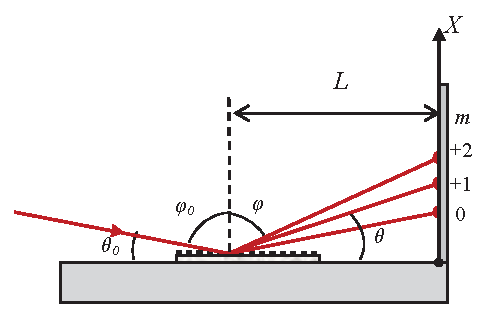
\includegraphics[width=7cm,height=4cm]{pic1.pdf}{\label{1}}}
				\ffigbox[\FBwidth]{\caption{}}%
				{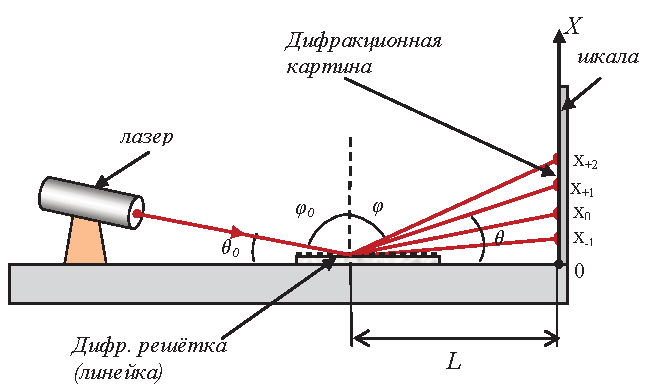
\includegraphics[width=7cm,height=4cm]{pic2.pdf}}         
			\end{subfloatrow}
		}
		{\caption{Схема установки.}}{\label{fig:pic}}
	\end{figure}


\section{Экспериментальная часть}
	\subsection{Порядок выполнения работы}
		\begin{enumerate}
			\item
				Собираем установку: крепим лазер под небольшим углом как показано на рис.~\ref{fig:pic}, светим на полумиллиметровую шкалу линейки, сама линейка расположена на $L$, от стены, где в дальнейшем будет наблюдаться дифракционная картина.
			\item 
				На маркерной доске отмечаем максимумы, также записываем харкатерные размеры системы и находим угол падения луча лазера на линейку. Далее измеряем расстояния от нулевого максимума до каждого из последующих максимумов.
			\item 
				Измерения проведём для двух разных углов.
		\end{enumerate}
	
	\subsection{Экспериментальные данные}
		\floatsetup[table]{capposition=top}	
		\begin{table}[H]
			\caption{Некоторые измеряемые величины и их погрешность.}
			\label{table:parametr}
			\begin{tabular}{|c|c|c|c|c|}
				\hline
				& $L$, см & $\Delta x$, см & $x_0^{(1)}$, см & $x_0^{(2)}$, см \\ \hline
				Величина          & 98      & 10,0           & 4,0             & 7,5             \\ \hline
				Погрешность       & 0,2     & 0,2            & 0,2             & 0,2             \\ \hline
				$\varepsilon$, \% & 0,2     & 2              & 5               & 3             \\ \hline
			\end{tabular}
		\end{table}
	
		\floatsetup[table]{capposition=top}	
		\begin{table}[H]
			\caption{Результаты измерений.}
			\label{table:exp}
			\begin{tabular}{|c|c|c|c|c|c|c|}
				\hline
				& \multicolumn{3}{c|}{№ 1}                          & \multicolumn{3}{c|}{№ 2}                          \\ \hline
				$m$ & $\Delta x$, см & $x_m^2-x_0^2$, см$^2$ & $\sigma$, см$^2$ & $\Delta x$, см & $x_m^2-x_0^2$, см$^2$ & $\sigma$, см$^2$ \\ \hline
				0   & 0,0            & 0                     & --       & 0,0            & 0                     & --       \\ \hline
				1   & 2,0            & 20                    & 3        & 1,3            & 21                    & 4        \\ \hline
				2   & 3,3            & 37                    & 3        & 2,3            & 40                    & 4        \\ \hline
				3   & 4,3            & 53                    & 4        & 3,3            & 60                    & 5        \\ \hline
				4   & 5,4            & 72                    & 5        & 4,2            & 81                    & 5        \\ \hline
				5   & 6,3            & 90                    & 6        & 5,1            & 103                   & 6        \\ \hline
				6   & 7,2            & 109                   & 6        & 5,8            & 121                   & 6        \\ \hline
				7   & 8,0            & 128                   & 7        & 6,6            & 143                   & 7        \\ \hline
				8   & 8,8            & 148                   & 7        & 7,3            & 163                   & 7        \\ \hline
				9   & 9,5            & 166                   & 8        & 8,0            & 184                   & 8        \\ \hline
				10  & 10,1           & 183                   & 8        & 8,6            & 203                   & 8        \\ \hline
				11  & 10,8           & 203                   & 9        & 9,2            & 223                   & 8        \\ \hline
				12  & 11,3           & 218                   & 9        & 10,0           & 250                   & 9        \\ \hline
				13  & 11,9           & 237                   & 10       & 10,5           & 268                   & 9        \\ \hline
				14  & 12,6           & 260                   & 10       & 11,0           & 286                   & 10       \\ \hline
				15  & 13,1           & 276                   & 11       & 11,5           & 305                   & 10       \\ \hline
				16  & 13,7           & 297                   & 11       & 12,1           & 328                   & 11       \\ \hline
				17  & 14,2           & 315                   & 12       & 12,6           & 348                   & 11       \\ \hline
				18  & 14,8           & 337                   & 12       &                &                       &          \\ \hline
				19  & 15,3           & 356                   & 12       &                &                       &          \\ \hline
				20  & 15,9           & 380                   & 13       &                &                       &          \\ \hline
				21  & 16,4           & 400                   & 13       &                &                       &          \\ \hline
				22  & 16,9           & 421                   & 14       &                &                       &          \\ \hline
				23  & 17,4           & 442                   & 14       &                &                       &          \\ \hline
			\end{tabular}
		\end{table}
	
	\newpage
	\subsection{Обработка результатов}
		На основани результатов измерений, представленных в таблице~\ref{table:exp}, построим интерполяционные прямые, иллистрирующие зависимости $x_m^2-x_0^2$, см$^2$ от $m$ для двух серий эксперимента.
		\begin{figure}[h!]
			\begin{floatrow}
				\ffigbox[\FBwidth]{\caption{Зависимость $x_m^2-x_0^2$, см$^2$ от $m$.}\label{fig:Graph_1}}%
				{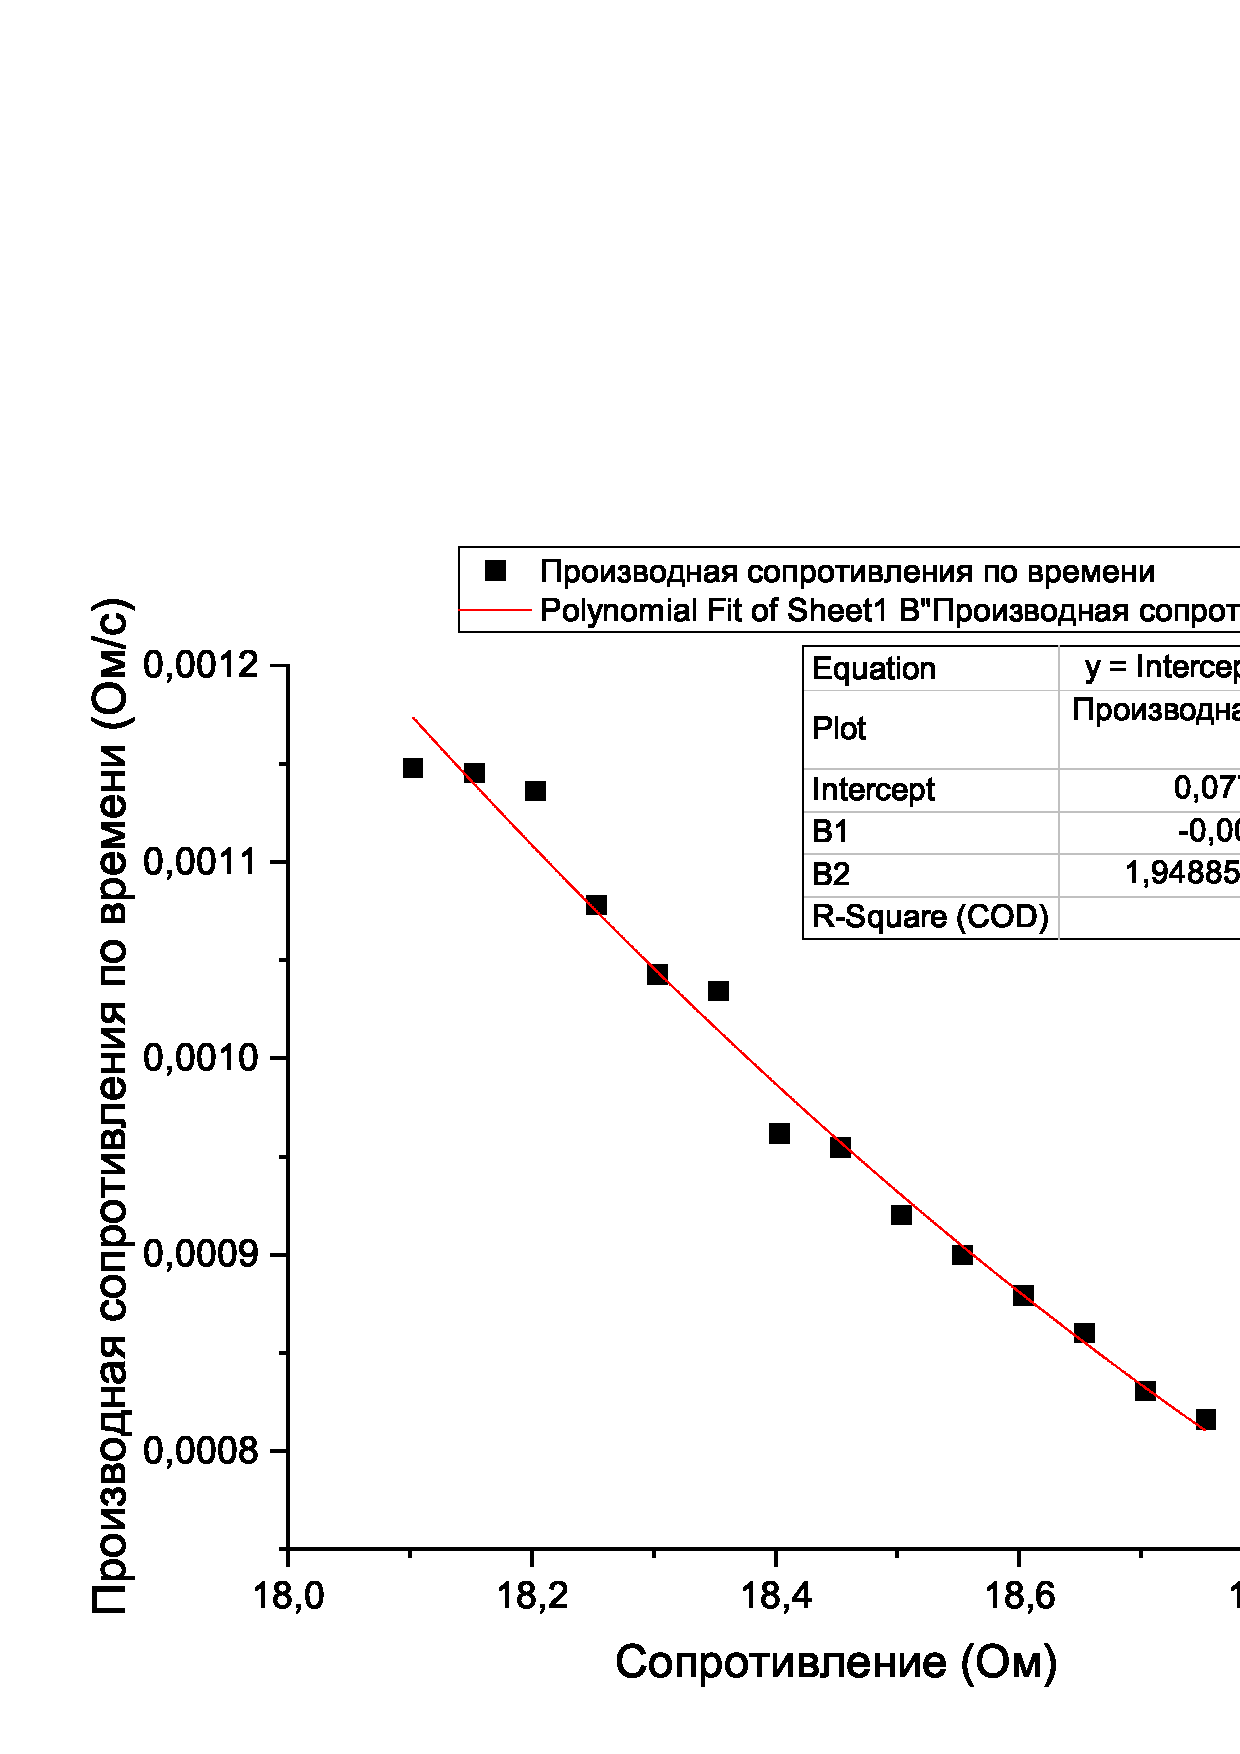
\includegraphics[width=8cm,height=7cm]{Graph1}}
				\ffigbox[\FBwidth]{\caption{Зависимость $x_m^2-x_0^2$, см$^2$ от $m$.}\label{fig:Graph_2}}%
				{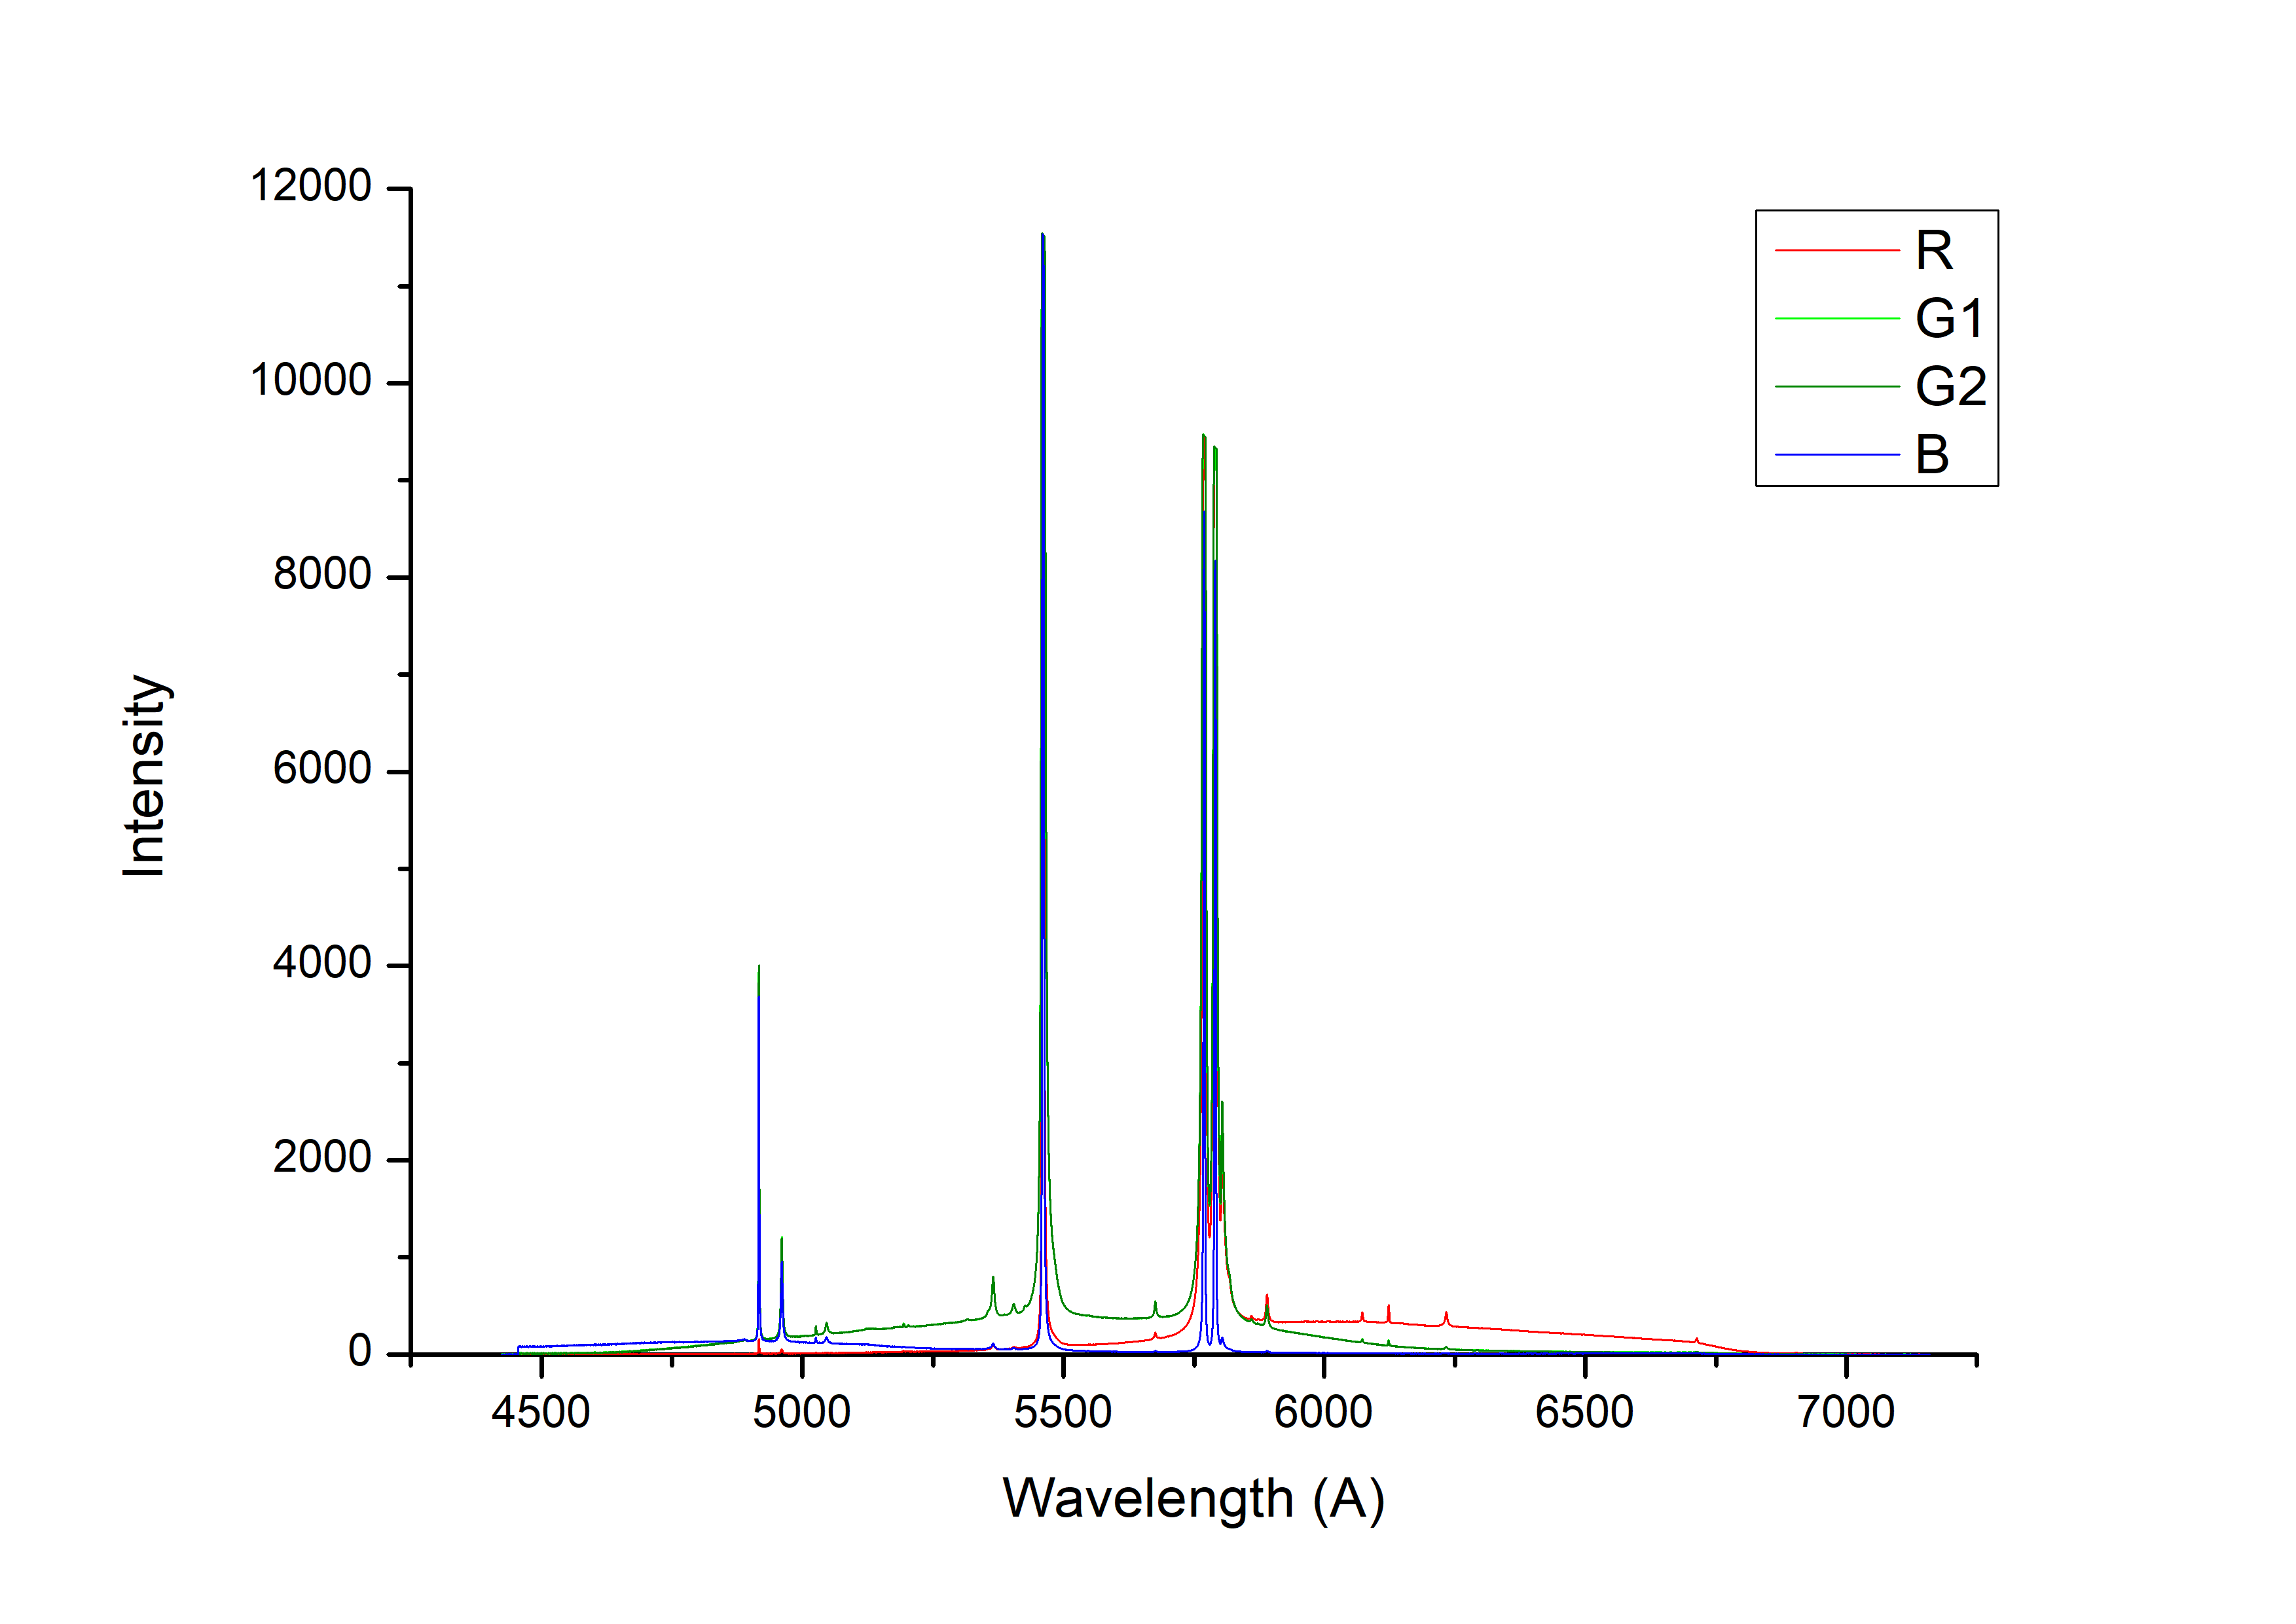
\includegraphics[width=8cm,height=7cm]{Graph2}}         
			\end{floatrow}
		\end{figure}
		
		В таблице \ref{k} представлены значения наклонов графиков, изображенных на рисунках \ref{fig:Graph_1} и \ref{fig:Graph_2}, а в таблице~\ref{lambda} представлены результаты расчета длины волны лазера по формуле (\ref{formula}). Погрешность результата можно оценить следующим образом: $\sigma_\lambda = \lambda \frac{\sigma_\beta}{\beta}$.
		
		\begin{table}[h!]
			\begin{floatrow}
				\ttabbox[\FBwidth]{\caption{$\beta$.}\label{k}}%
				{\begin{tabular}{|c|c|c|}
						\hline
						& $\beta$, см$^2$ & $\sigma_\beta$, см$^2$ \\ \hline
						1 & 18,73           & 0,11                   \\ \hline
						2 & 20,47           & 0,07                   \\ \hline
				\end{tabular}}
				\ttabbox[\FBwidth]{\caption{$\lambda$.}\label{lambda}}%
				{\begin{tabular}{|c|c|c|}
						\hline
						& $\lambda$, нм & $\sigma_\lambda$, нм \\ \hline
						1 & 489           & 3                    \\ \hline
						2 & 533           & 2                    \\ \hline
				\end{tabular}}        
			\end{floatrow}
		\end{table}

\section{Выводы}
	В ходе лабораторной работы мы наблюдали интерференционная картину, полученную на грубой дифракционной решетке ($\lambda \ll d $), а именно на металлической линейке. 
	
	По распределению максимумов на экране мы определили длину волны зеленого лазера. Для повышения точности результатов эксперимент был проведен два раза. Во втором случае длина волны лазера получилась равной 533 нм с относительной погрешностью 0,4\%, что достаточно точно совпадает с паспортным значением -- 532 нм. В первом же эксперименте результат оказался заниженным -- 489 нм. Это может быть связано с тем, что луч лазера, падая на дифракционную решетку под скользящим углом, создает протяженную размытую полосу света на линейке. То есть значение $L$ является грубо измеренной величиной. Так как из формулы~(\ref{formula}) следует, что $\lambda$ зависит квадратично от $1/L$, то малые изменения $L$ будут приводить к большой погрешности измерений.
	
	Увеличнение количества серий измерений приведет к понижению случайной ошибки, обусловленной расстоянием $L$.



	
\end{document}